\documentclass[11pt]{amsart}

\usepackage[a4paper,margin=1in]{geometry}
\usepackage{microtype}
\usepackage{amsmath,amssymb,amsthm,mathtools}
\usepackage{graphicx}
\usepackage{booktabs}
\usepackage[colorlinks=true,linkcolor=blue,citecolor=blue,urlcolor=blue]{hyperref}

\title{Results: KL Regularization against an EMA Reference}
\author{Brian Bartoldson}
\date{}

\newcommand{\R}{\mathbb{R}}
\newcommand{\E}{\mathbb{E}}
\newcommand{\KL}{\mathrm{KL}}
\newcommand{\Tn}{T_n}
\newcommand{\En}{E_n}
\newcommand{\Tinf}{T_{n-\Delta}}
\newcommand{\klexact}{\log \Tn(y) - \log \En(y)}
\newcommand{\klapprox}{\tfrac{\alpha}{\Delta(1-\alpha)}\,\bigl(\log \Tn(y) - \log \Tinf(y)\bigr)}

\begin{document}
\maketitle

\section{Setup}

We train Qwen3-4B-Instruct-2507 with TBA on Countdown using asynchronous rollouts ($\Delta = 10$), $\alpha=0.9$ for the EMA reference, $\beta=0.005$, $\text{lr}=10^{-6}$, $K=16$ samples per problem, sequence length $4096$, $720$ training steps, evaluation every $20$ steps.

\paragraph{Per-token KL.}
Two choices for the per-token KL contribution to the advantage:
\begin{itemize}
    \item \emph{Exact KL:} $\;\klexact$, where $\En$ is the EMA reference policy.
    \item \emph{Approx KL:} $\;\klapprox$, the first-order surrogate derived in \texttt{main.tex} (eq.~2.10). This avoids a forward pass through $\En$ at training time.
\end{itemize}

\paragraph{Centering.}
For each rollout, the per-token KL is summed over masked tokens to give a per-rollout KL term $K^{(i)}$. The advantage is then adjusted by
\begin{equation}\label{eq:adv-update}
    \text{advantage}^{(i)} \;\mathrel{+}{=}\; -\beta \cdot \bigl(K^{(i)} - \bar{K}\bigr),
\end{equation}
where $\bar{K}$ is a centering term. Two choices:
\begin{itemize}
    \item \emph{K-centered:} $\bar{K}$ is the mean of $\{K^{(j)}\}_{j=1}^K$ over the $K$ rollouts that share a problem.
    \item \emph{No centering:} $\bar{K} \equiv 0$, so $\text{advantage}^{(i)} \mathrel{+}{=} -\beta K^{(i)}$ directly.
\end{itemize}

\section{$2\times 2$ matrix: EMA reference}

Crossing the two per-token KL choices with the two centering choices yields four cells:

\begin{center}
\begin{tabular}{lll}
\toprule
Cell & Per-sample KL formula & Centering \\
\midrule
Exact, K-centered      & $\klexact$ & $\bar{K}$ from same formula \\
Exact, no centering    & $\klexact$ & $\bar{K} = 0$ \\
Approx, K-centered     & $\klapprox$ & $\bar{K}$ from same formula \\
Approx, no centering   & $\klapprox$ & $\bar{K} = 0$ \\
\bottomrule
\end{tabular}
\end{center}

\begin{figure}[ht]
  \centering
  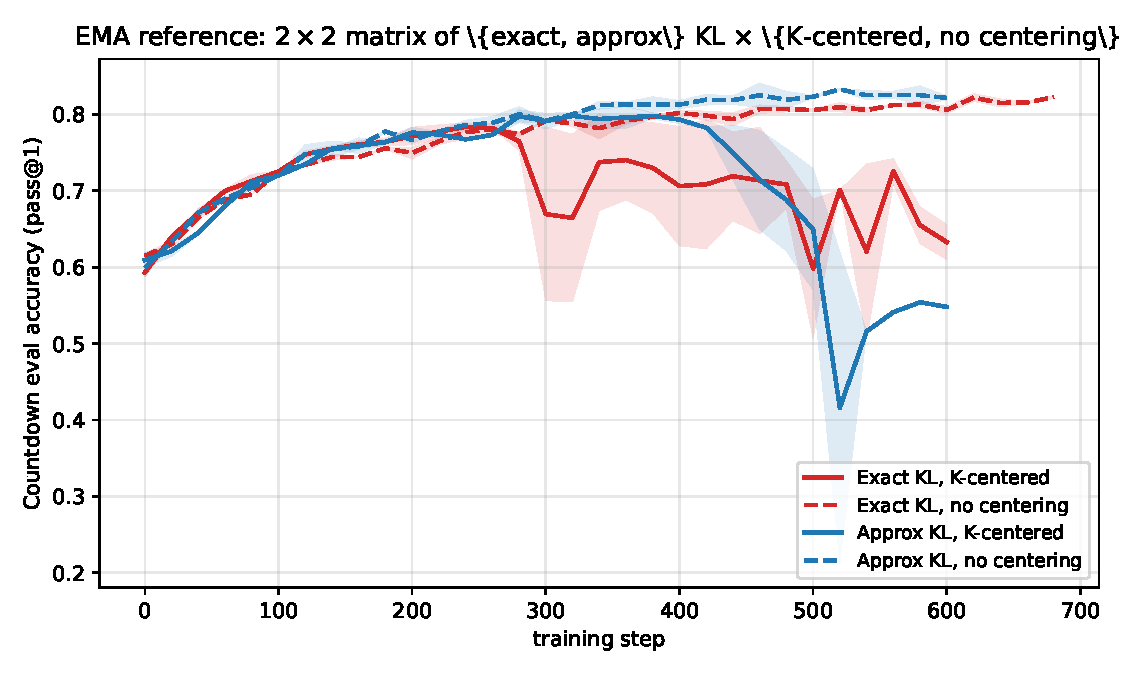
\includegraphics[width=0.95\linewidth]{fig_matrix.pdf}
  \caption{Eval accuracy on Countdown for the four cells of the EMA-reference matrix. Red: exact KL. Blue: approx KL. Solid: K-centered. Dashed: no centering. The two no-centering cells (dashed) plateau above $0.80$ and peak above $0.82$; the two K-centered cells (solid) peak earlier and degrade after step $\approx 300$.}
  \label{fig:matrix}
\end{figure}

\begin{center}
\begin{tabular}{lcc}
\toprule
Cell & Peak eval (step) & Final eval \\
\midrule
Exact, K-centered    & $0.789$ (240) & $0.656$ \\
Exact, no centering  & $\mathbf{0.827}$ (620) & $0.821$ \\
Approx, K-centered   & $0.794$ (380) & $0.548$ \\
Approx, no centering & $\mathbf{0.831}$ (520) & $0.819$ \\
\bottomrule
\end{tabular}
\end{center}

The headline observations:
\begin{enumerate}
  \item Within either KL choice, removing the centering term strictly helps.
  \item The approx-KL row tracks the exact-KL row closely: peaks differ by $0.005$ and finals by $0.002$ in the no-centering pair. This is the empirical justification for substituting the first-order surrogate (no extra forward) for the exact EMA KL.
  \item The K-centered cells exhibit the same kind of late-run instability under both per-token KL choices, suggesting the failure mode is centering-related rather than KL-formula-related.
\end{enumerate}

\section{Reset reference (baseline)}

Before the EMA work, the same kinds of variants were tested with a reset reference policy (hard copy from the training policy every $50$ rollout steps). Reset-ref runs use the \emph{exact} KL only (the approximation requires an EMA), and explore three choices for where to obtain $\log\Tn$ in the per-sample term and in the K-group mean. Naming below: ``inf-mean'' / ``train-mean'' indicates which source is used for $\log\Tn$ in the K-group mean.

\begin{center}
\begin{tabular}{lll}
\toprule
Run & Per-sample KL ($\log\Tn$ from) & K-group mean ($\log\Tn$ from) \\
\midrule
Exact KL, K-centered (inf-mean)   & live train forward & inference snapshot \\
Exact KL, K-centered (train-mean) & live train forward & live train forward \\
Inf-snapshot KL, K-centered (inf-mean) & inference snapshot & inference snapshot \\
\bottomrule
\end{tabular}
\end{center}

Each of the three is run with and without importance sampling, for six total curves in Figure~\ref{fig:reset}.

\begin{figure}[ht]
  \centering
  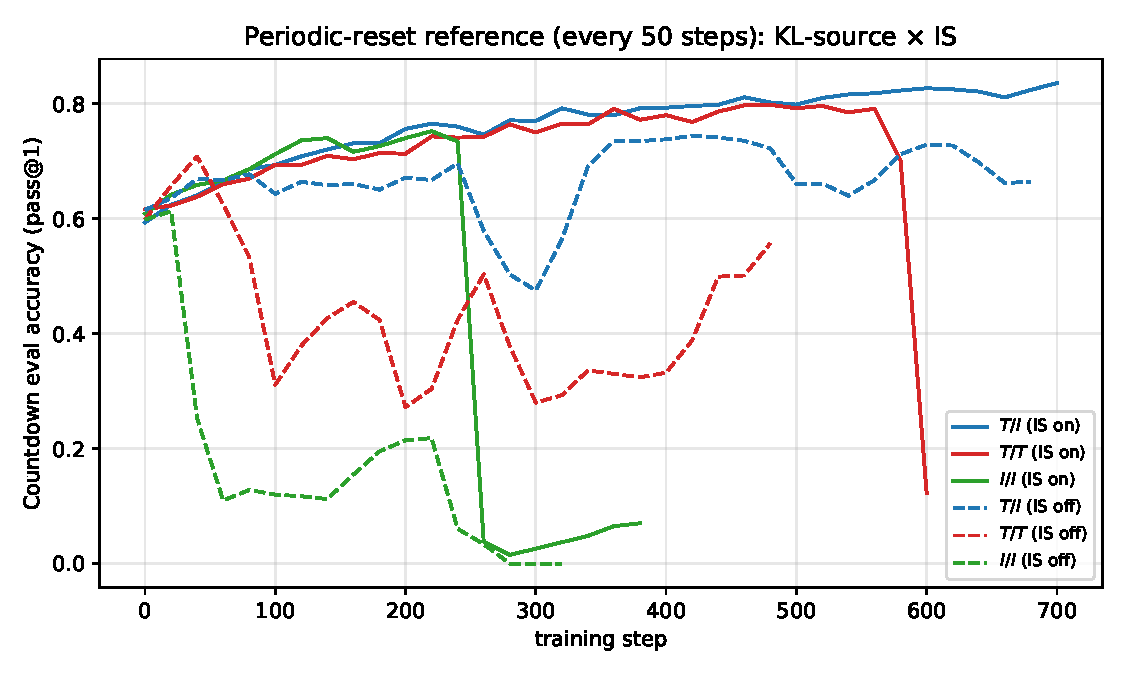
\includegraphics[width=0.95\linewidth]{fig_reset.pdf}
  \caption{Eval accuracy on Countdown with periodic-reset reference. Both \emph{Exact KL, K-centered (train-mean)} variants (red) collapse late in training; the \emph{Inf-snapshot} variant (green) without IS gets stuck at zero; only the \emph{Exact KL, K-centered (inf-mean)} variants (blue) trained stably.}
  \label{fig:reset}
\end{figure}

\begin{center}
\begin{tabular}{lcc}
\toprule
Run & Peak eval (step) & Final eval \\
\midrule
Exact KL, K-centered (inf-mean)        & $0.836$ (700) & $0.836$ \\
Exact KL, K-centered (train-mean)      & $0.798$ (480) & $0.122$ \\
Inf-snapshot KL, K-centered (inf-mean) & $0.752$ (220) & $0.070$ \\
Exact KL, K-centered (inf-mean) no IS  & $0.744$ (680) & $0.664$ \\
Exact KL, K-centered (train-mean) no IS & $0.708$ (40) & $0.557$ \\
Inf-snapshot KL, K-centered (inf-mean) no IS & $0.613$ (20) & $0.000$ \\
\bottomrule
\end{tabular}
\end{center}

The train-mean centering instability under reset reference mirrors the K-centered instability in the EMA matrix.

\section{Approximation accuracy}

We track the per-token error of the first-order surrogate against the exact EMA KL inside \texttt{tba\_loss}: \texttt{MAE} (mean absolute error over masked tokens) and \texttt{bias} (signed mean). Figure~\ref{fig:approx-error} compares the two no-centering cells (where the loss path differs but both have the same telemetry).

\begin{figure}[ht]
  \centering
  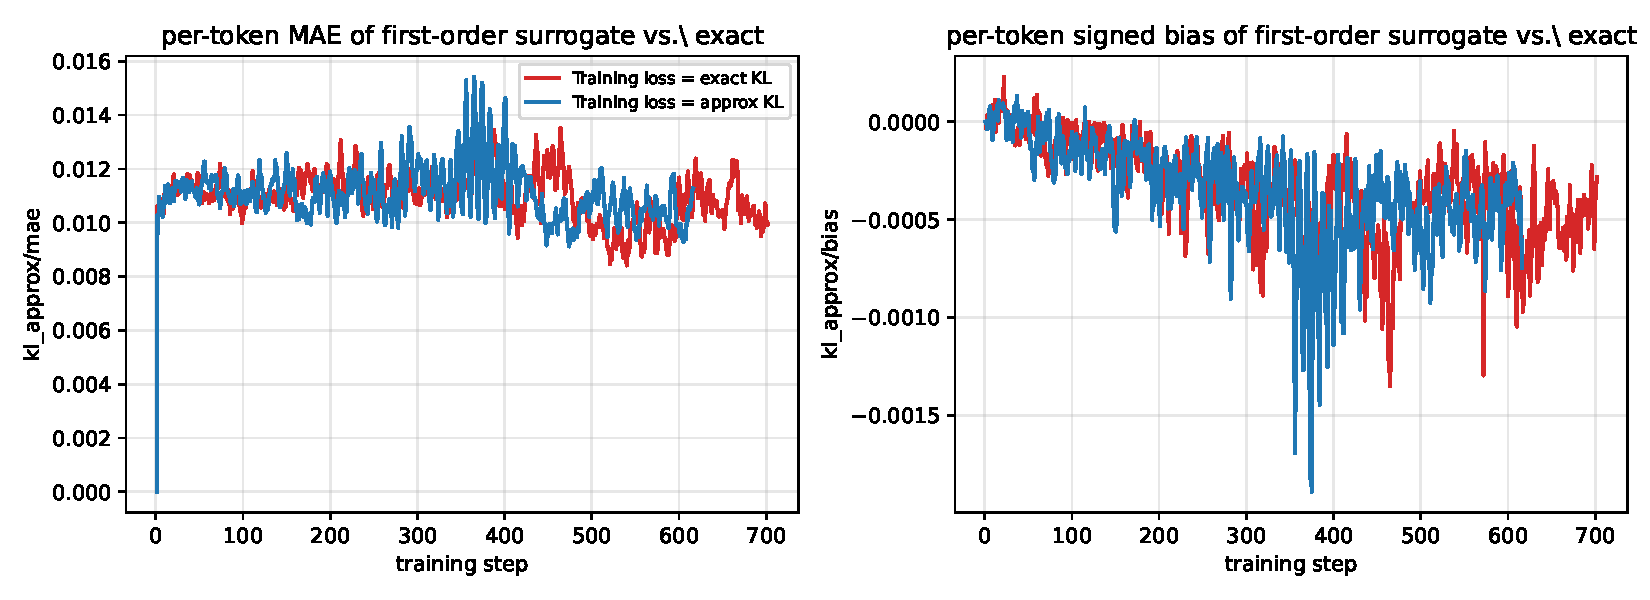
\includegraphics[width=0.98\linewidth]{fig_approx_error.pdf}
  \caption{Per-token MAE (left) and signed bias (right) of the first-order surrogate $\klapprox$ against the exact $\klexact$, computed over masked tokens within each rollout. Both no-centering cells: red uses the exact KL in the loss; blue uses the approx KL in the loss.}
  \label{fig:approx-error}
\end{figure}

MAE stays in the low $10^{-2}$ band throughout training, and the signed bias is at most a few parts in $10^{3}$. The approximation is empirically faithful, regardless of whether it is used in the loss.

\section{Conclusion}

Removing the K-group centering is the dominant lever: both EMA exact and EMA approx benefit. With centering off, the cheap first-order surrogate matches the exact EMA KL within $0.005$ on peak eval and $0.002$ on final eval, so it is a viable drop-in replacement that saves a forward pass through the reference model.

\end{document}
